\documentclass[12pt]{article}
\usepackage{times}
\usepackage{geometry}
\usepackage[english]{babel}
\usepackage[utf8]{inputenc}
\usepackage{fancyhdr}
\usepackage{graphicx}
\usepackage{titlesec}
\usepackage{biblatex}
\usepackage{minted}
\usepackage{xcolor} % to access the named colour LightGray
\definecolor{LightGray}{gray}{0.9}



\setlength{\headheight}{15.2pt}
\setcounter{secnumdepth}{3}
\rfoot{Pg: \thepage}

\geometry{
   a4paper,
   left = 25mm,
   top = 20mm,
}
\begin{document}
\thispagestyle{empty}

\section*{}
 {\LARGE\makebox[\textwidth]{\textbf{KATHMANDU UNIVERSITY}}}

\centerline{Department of Computer Science and Engineering}
\centerline{Dhulikhel,Kavre}
\begin{figure}[h]
    \centerline{
\includegraphics[width=50.546mm,height=50.546mm]{KU_Logo.png}}
\end{figure}

\centerline{\textbf{A Project Report}}
\centerline{on}
\centerline{\underline{\textbf{"Tic Tac Toe"}}}

\vspace*{12mm}

\centerline{\textbf{[Code No. : COMP 342]}}
\centerline{(For partial fulfillment of 3rd Year/ 1st Semester in Computer Science)}

\vspace*{20mm}

\centerline{\textbf{Submitted by}}
\centerline{\textbf{Aayush Pokharel (Roll No. 43)}}
\centerline{\textbf{Dikshya Poudel (Roll No. 45)}}


\vspace*{26mm}


\centerline{\textbf{Submitted to}}
\centerline{\textbf{Dhiraj Shrestha}}
\centerline{\textbf{Dept of Computer Science and Engineering}}

\vspace*{20mm}

\centerline{\textbf{Submission Date: 20th December, 2022}}



\clearpage
\thispagestyle{empty}

\section*{Abstract}
The project report for the mini project "Tic Tac Toe" is drafted to meet the prerequisites to partially fulfill
the COMP 342 course offered by the Department of Computer Science and Engineering at Kathmandu University.
This project was designed with the objective to teach the OpenGL rendering pipeline in a practical manner to the students enrolled in
COMP 342 course.\\\\
We the involved project members decided to utilize PyOpenGL, a Python wrapper library for OpenGL's API, and PyGame to create a small pixel-perfect game having a resolution of 800x800 pixels
to meet the requirements of the course. Keeping the restriction of only using OpenGL for rendering, we forgo PyGame's abstracted library functions
for rendering and used PyOpenGL to render the graphics in the PyGame window under a double buffer system.
PyGame however was used to code the game logic, loops, and windowing tasks.\\\\
For the application, the grid lines to make the tic tac toe board was rendered, and then via appending the vertices list, later on, rebinding the updated buffer and redrawing it, user input was rendered.
\\\\
\textbf{Keywords: }OpenGL, PyGame, PyOpenGL,

\clearpage
\thispagestyle{empty}
\tableofcontents

\clearpage
\thispagestyle{empty}
\listoffigures

\clearpage
\pagenumbering{arabic}
\section{CHAPTER 1: INTRODUCTION}
Tic tac toe is a two players game where they alternately mark the squares in a three-by-three grid with an X or an O.
In it, the player who successfully arranges three of their marks in a row that is either horizontal, vertical, or diagonal
is declared the winner. In our project, we have implemented a small pixel-perfect game 'tic tac toe' having a resolution of
800x800 pixels by utilizing PyOpenGL for OpenGL’s API and PyGame. \\\\
OpenGL (Open Graphics Library) is a cross-language, cross-platform application programming interface (API) for rendering 2D
and 3D vector graphics. The API is typically used to interact with a GPU, to achieve hardware-accelerated rendering. It is
commonly used to make 3d model viewers and animations more responsive as well as to handle embedded video or to draw vector graphics.
PyGame is a cross-platform set of Python modules designed for writing video games. It includes computer graphics and sound libraries
designed to be used with the Python programming language.
We have used PyOpenGL to bind Python to OpenGL and related APIs using provided library functions

\subsection{Objectives}
The main objective of this project is to understand the concepts of the OpenGL Rendering pipeline and utilize the knowledge to create a practical example to enhance our knowledge to solve real-life problems. Besides, the other objectives are listed below:
\begin{itemize}
    \item To create a playable multiplayer game.
    \item To learn how python data types can be used in to make a python script communicate with a C library.
    \item To explore the Desktop app creation process.
\end{itemize}

\subsection{Motivation and Significance}
The main motivation behind this project is to learn the fundamentals and working procedures of the OpenGL rendering pipeline in a fun and entertaining manner. Furthermore, the noble idea of becoming a game developer and utilizing the concepts discussed in
a Kathmandu University Open Source Society (KUOSC)'s game dev workshop solidified the idea to make the Tic Tac Toe game.
\clearpage
\section{CHAPTER 2: PROJECT DETAILS}
The project is a simple game and only has one window that accepts the mouse input to draw the 2D shapes.\\


\begin{figure}[h]
    \centerline{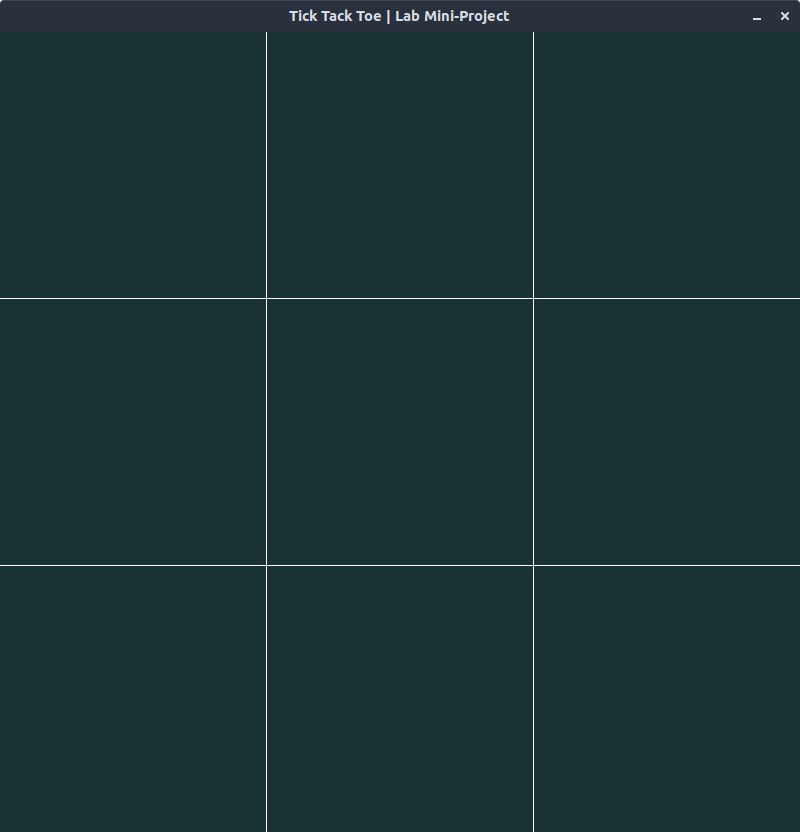
\includegraphics[height=80mm]{InitialWindow.png}}
    \caption{Application's Window}
    \label{fig}
\end{figure}

The project can mainly be divided into three parts. These three parts are each handled by their respective classes. The classes are as follows:
\begin{itemize}
    \item App
    \item BackgroundLines
    \item GameState
\end{itemize}

\clearpage
\begin{figure}[h]
    \centerline{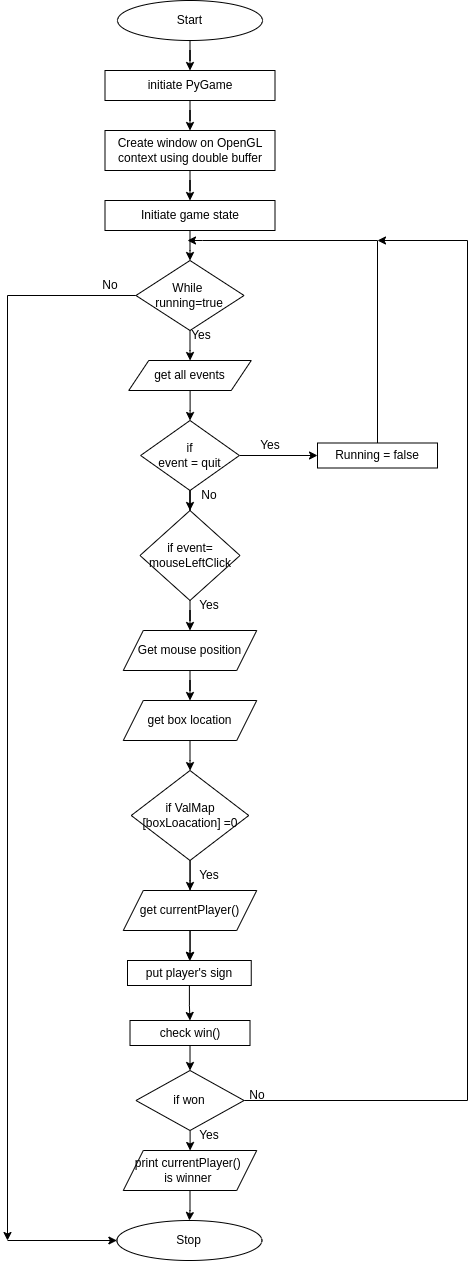
\includegraphics[height=200mm]{TicTacToeHighLevelFlowchart.png}}
    \caption{Overview of the Application}
    \label{fig}
\end{figure}

\clearpage

\subsection{App}
The App class is the main class for the application. It is responsible for the whole cycle of the application. Its task is to create a PyGame Window, manage the rendering and window creation along with keeping the  infinite game loop (here, named the main loop) running as long as the application is running, and to break the loop when
the exit condition is provided.\\\\
Further more the App class instantiates the other two classes and makes use of them. It also handles the user input (here, especially mouse input).\\\\
The app class has the following methods:
\begin{itemize}
    \item \textbf{\_\_init\_\_(self)}\\ This is the constructor of the application and it handles all the instantiation and initial setting of the variables.
    \item \textbf{createShader(self, vertexFilePath, fragmentFilePath)}\\ The modern OpenGl pipeline is to use programmable shaders written in GLSL (OpenGL Shading Language). This function reads the text file which contains the shaders and compiles the vertex and fragment shader and returns it in a usable format by the rest of the application.
    \item \textbf{mainLoop(self)}\\ This is the main loop of the application. It runs infinitely until its breaking condition is given. It is responsible for initially drawing the buffer and periodically updating it. It also listens to the user Inputs and acts upon them. When faced with a mouse click, this class gets the pixel location of the mouse and calls the necessary function to determine on which box the mouse is currently on. It also checks if there are any changes to the Game Board's states and on changes it calls the necessary function to append the player's symbols vertices, extend the buffer and draw it.
    \item \textbf{quit(self)}\\ This is a deconstructor that is responsible for calling the deconstructor for the BackgroundLines class, deleting the compiled shader program, and quitting the PyGame window.
\end{itemize}
\clearpage
\subsection{BackgroundLines}
The BackgroundLine class is the class responsible for the drawing of the vertices on the window and the OpenGL rendering pipeline. It has an attribute named \textbf{vertices} which is a list that contains the vertices that bind to the Array Buffer and are used to render the line. We initially draw the gridlines to make the 'tic tac toe' board and
then dynamically append the vertices to create the user input-related shapes.
\\\\
The BackgroundLines class has the following methods:
\begin{itemize}
    \item \textbf{\_\_init\_\_(self)}\\ This is the constructor of the application and it handles all the instantiation and initial binding of the array to the Buffer.
    \item \textbf{getNewLine(self,val,cPlayer)}\\ This is the function that takes a reference to the boxes on which the mouse button was clicked and the current player and returns a list containing the vertices to their's corresponding input. For example, if playerX clicks on the area of the top-left box, this function checks the box and the current player and returns the list containing the vertices to draw an X on the top-left box.
    \item \textbf{addNew(self,lis)}\\This function accepts the dynamically generated list, converts it to a numpy array (because OpenGL doesn't understand Python Lists), and recreates the buffer with the updated array and binds it so that the vertices could be rendered by the OpenGL.
    \item \textbf{destroy(self)}\\ This is a deconstructor that is responsible for clearing up the Vertex Array and deleting the Buffer after use.
\end{itemize}
\begin{figure}[h]
    \centerline{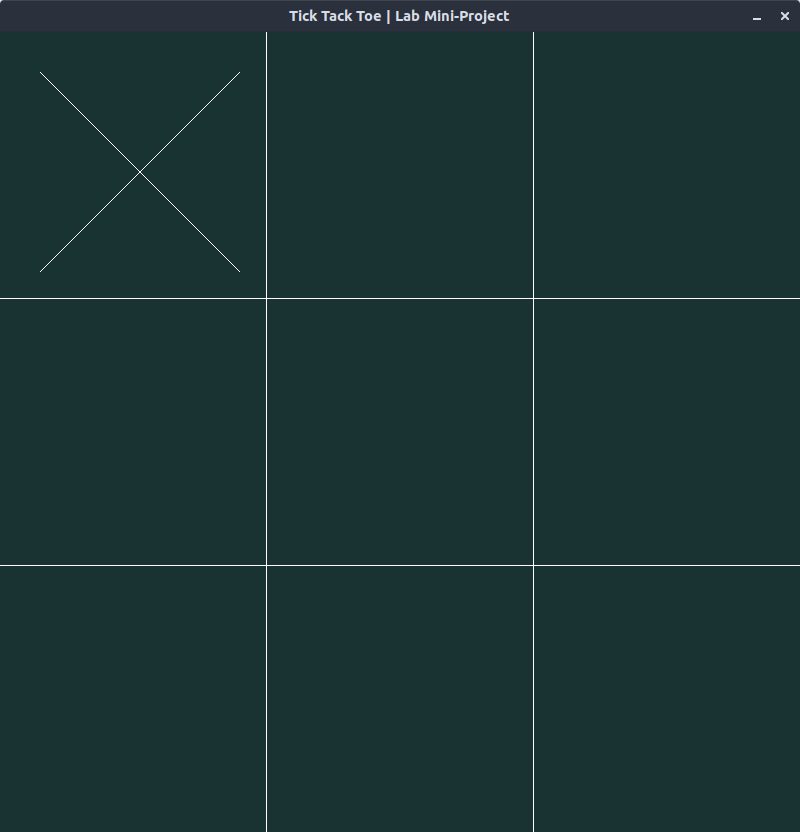
\includegraphics[height=80mm]{userInput.png}}
    \caption{Drawing shapes after PlayerX's input}
    \label{fig}
\end{figure}
\begin{figure}[h]
    \centerline{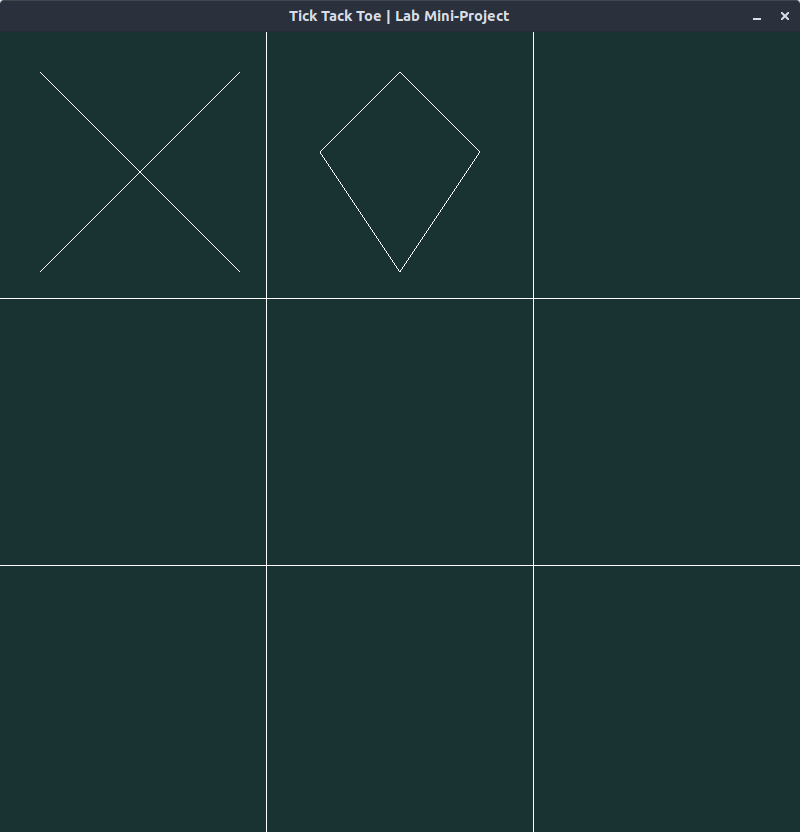
\includegraphics[height=80mm]{userInput2.png}}
    \caption{Drawing shapes after PlayerO's input}
    \label{fig}
\end{figure}

\subsection{GameState}
The GameState class is a decoupled class that is responsible for most of the game logic. It doesn't care about the rendering pipeline or any
kind of buffer. It plainly runs under the game loop and keeps track of the game's state and provides methods to implement various game logic.
\\\\
The app has the following methods:
\begin{itemize}
    \item \textbf{\_\_init\_\_(self)}\\ This is the constructor of the GameState and it handles setting the game's variables to initial values.
    \item \textbf{getCurrentPlayer(self)}\\ This returns the current player who has the current turn.
    \item \textbf{putValue(self,positionBox)}\\ This is the most important function in terms of the game logic in the application. It takes a refrence to the box position and checks if it's empty (if the ValMap at the given index is 0, it signifies that it's empty); checks who the current player is and changes the value at reference location with the players' value ( 1 for X and 2 for O) and finally checks if the player's input has triggered a win condition.
    \item \textbf{checkIfSameValue(self,val1,val2,val3)}\\ This is a function that takes three values and checks the indexes of ValMap referenced by those values to see if the three values are all same. It returns a string "X Wins" if it matches three 1s and "O Wins" if it matches three 2s.
    \item \textbf{checkHorizontal(self)}\\ This function is used to check the three horizontal rows to see if any of them trigger a win condition.
    \item \textbf{checkVertical(self)}\\ This function is used to check the three vertical columns to see if any of them trigger a win condition.
    \item \textbf{checkDiagonal(self)}\\ This function is used to check the two diagonals to see if any of them trigger a win condition.
    \item \textbf{checksLoc(self,xLoc,yLoc)}\\ This function takes in the pixel position of the mouse click and compares it with the bounding limits of the nine boxes to see on which box the mouse pointer clicked on.
    \item \textbf{checkWin(self)}\\ This function is used to encapsulate all the calls to check the win conditions. It returns the value of \textbf{self.won} .
    \item \textbf{printBoardCondition(self,con)}\\ This function takes a string and prints the board condition to the console in 3x3 matrix order. It was extensively used during development to keep track of the board's state and debug input logic.
\end{itemize}


\section{CHAPTER 3: CONCLUSION}
OpenGL serves as an important stepping stone for venturing into the field of Computer Graphics Design and Application. This project has enabled us to work with mid-level OpenGL complexity. We have extensively documented the work of each function call and variable used in the project for better understanding. Hence, developing a simple game 'Tic tac toe' has demonstrated the usefulness of the OpenGL platform for low-cost and simple game development.
\subsection{Problems Encountered}
The following issues were encountered during the game development process:
\begin{itemize}
    \item As OpenGL is not an UI Library, an user-friendly UI couldn't be created.
    \item It was too complicated to render text using OpenGL due to which we get a white blank window screen on 'Win' condition.
\end{itemize}
\subsection{Future Enhancements}
The following actions could be taken to improve the program:
\begin{itemize}
    \item We can make the UI simple and more user-friendly.
    \item We can add the functionality of 'Redo' and 'Undo' to the program.
    \item We can display the winner's name in the window screen after a player wins.
    \item We can add a replay function.
\end{itemize}

\clearpage

\section{VIDEO DEMONSTRATION}
\begin{itemize}
    \item Environment Setup\\
          \url{https://drive.google.com/file/d/12uOjQp0a1VumHvTVa8jk84nolvt9Oxm4/view?usp=sharing}
    \item Application Demo\\
          \url{https://drive.google.com/file/d/1Yty0j2IKSQPJlEcB27bdLMEo6geNegG_/view?usp=sharing}
\end{itemize}

\section{SOURCE CODE}
\textbf{The Repository for this project can be found at }\\\\ \url{https://github.com/AayushPokharel/CG_Lab/tree/main/Lab_Project}
\clearpage

\section{REFERENCES}
\begin{itemize}
    \item PyOpenGL Documentation.\\ \url{https://pyopengl.sourceforge.net/documentation/index.html?}

    \item OpenGL® 4.5 Reference Pages.\\ \url{https://registry.khronos.org/OpenGL-Refpages/gl4/?}

    \item PyGame.\\
          \url{https://devdocs.io/pygame/}
\end{itemize}

\end{document}